\documentclass[tikz,border=3.14mm]{standalone}
\usetikzlibrary{shadings}
\usepackage{pgfplots}
\pgfplotsset{compat=1.16}
\begin{document}
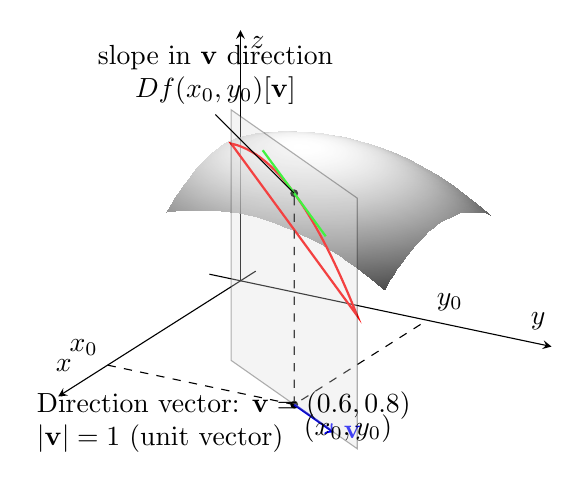
\begin{tikzpicture}[bullet/.style={circle,fill,inner sep=1pt},
 declare function={f(\x,\y)=2-0.5*pow(\x-1.25,2)-0.5*pow(\y-1,2);
                  vx=0.6; vy=0.8;}] % Direction vector v = (0.6, 0.8), |v| = 1
 \begin{axis}[view={120}{30},colormap/blackwhite,axis lines=middle,%
    zmax=2.2,zmin=0,xmin=-0.2,xmax=2.4,ymin=-0.2,ymax=2,%
    xlabel=$x$,ylabel=$y$,zlabel=$z$,
    xtick=\empty,ytick=\empty,ztick=\empty]
  % Surface plot
  \addplot3[surf,shader=interp,domain=0.6:2,domain y=0.5:1.9,opacity=0.7] 
   {f(x,y)};
  
  % Curve along direction v through (x_0, y_0)
  \addplot3[thick,red,domain=-0.8:0.8,samples=50]  
   ({1.75+vx*x},{1.2+vy*x},{f(1.75+vx*x,1.2+vy*x)}); 
  
  % Point (x_0, y_0) and vertical line
  \draw[dashed] (1.75,0,0) node[above left]{$x_0$} -- (1.75,1.2,0)
  node[bullet] (b1) {}  -- (0,1.2,0) node[above right]{$y_0$}
  (1.75,1.2,0) -- (1.75,1.2,{f(1.75,1.2)})node[bullet] {};
  
  % Direction vector v in xy-plane
  \draw[->,thick,blue] (1.75,1.2,0) -- ({1.75+0.5*vx},{1.2+0.5*vy},0) 
   node[right] {$\mathbf{v}$};
  
  % Tangent line along directional derivative
  \draw[green,thick] ({1.75-0.4*vx},{1.2-0.4*vy},{f(1.75,1.2)-0.4*(-0.5*2*(1.75-1.25)*vx-0.5*2*(1.2-1)*vy)}) -- 
   ({1.75+0.4*vx},{1.2+0.4*vy},{f(1.75,1.2)+0.4*(-0.5*2*(1.75-1.25)*vx-0.5*2*(1.2-1)*vy)})
   coordinate[pos=0.5] (aux1);
  
  % Vertical plane containing the curve
  \draw[opacity=0.3,fill=gray!30] 
   ({1.75-0.8*vx},{1.2-0.8*vy},0) -- ({1.75+0.8*vx},{1.2+0.8*vy},0) --
   ({1.75+0.8*vx},{1.2+0.8*vy},2.2) -- ({1.75-0.8*vx},{1.2-0.8*vy},2.2) -- cycle;
   
 \end{axis}
 
 % Label for directional derivative
 \draw (aux1) -- ++ (-1,1) node[above,align=center]{slope in $\mathbf{v}$ direction\\
  $Df(x_0,y_0)[{\mathbf{v}}]$};
 \node[anchor=north west] at (b1) {$(x_0,y_0)$}; 
 
 % Legend for direction vector
 \node[anchor=south west,align=left] at (0,0) {
  Direction vector: $\mathbf{v} = (0.6, 0.8)$\\
  $|\mathbf{v}| = 1$ (unit vector)
 };
 
\end{tikzpicture}
\end{document}
